
\chapter{Graceful Degradation and Safe Landing}
\label{ch:graceful-degradation}

This chapter formalises the \emph{graceful degradation} property of the DC3S
safety shield and introduces the \emph{safe-landing} protocol: a sequence of
actions that guides the battery SOC toward a predefined safe zone when
observation quality drops below a critical threshold.

\section{Motivation}

When telemetry reliability~$w_t$ falls below a minimum threshold
$w_{\min}$, the DC3S shield cannot guarantee safety of any non-trivial
dispatch action.  Rather than halting abruptly (which may itself cause
grid imbalance), the system should \emph{land safely}: reduce dispatch
magnitude monotonically until SOC reaches a zone-centre value where
further degradation poses minimal risk.

\section{Safe-Landing Protocol}

\begin{definition}[Safe-landing trajectory]
\label{def:safe-landing}
A \emph{safe-landing trajectory} from state $x_t$ is a finite action
sequence $\{a_\tau\}_{\tau=t}^{t+T_L}$ such that:
\begin{enumerate}
  \item $|a_\tau| \le |a_{\tau-1}|$ for all $\tau$ (monotonic power reduction),
  \item $x_{t+T_L} \in \mathcal{X}_{\text{safe}} \coloneqq
    [\text{SOC}_{\min} + m,\, \text{SOC}_{\max} - m]$
    for margin $m > 0$, and
  \item each $a_\tau$ satisfies the SOC, power, and ramp constraints
    assuming worst-case load within the last-known uncertainty set.
\end{enumerate}
The landing time $T_L$ is the number of steps to reach $\mathcal{X}_{\text{safe}}$.
\end{definition}

\section{Landing Controller Design}

The landing controller is a receding-horizon projection:

\begin{enumerate}
  \item Compute the tightened action set $\mathcal{A}_t$ with the \emph{last valid}
    uncertainty set (since no new telemetry is trusted).
  \item Solve a one-step LP that minimises $|a_t|$ (net dispatch magnitude)
    subject to $a_t \in \mathcal{A}_t$ and the ramp constraint relative
    to the previous action.
  \item Apply the resulting action and repeat at $t+1$ with decaying
    uncertainty (the interval widens by the inflation factor each step
    without fresh calibration data).
\end{enumerate}

This controller is implemented in
\texttt{src/orius/dc3s/shield.py} via the
\texttt{repair\_action} function, which now exposes an explicit
\texttt{safe\_landing} mode and an optional low-reliability
auto-activation threshold.

\section{Experimental Evaluation}

We evaluate the landing protocol on two scenarios:

\subsection{Scenario 1: Sudden Blackout}
At step~$t = 72$ of a 168-hour \texttt{drift\_combo} episode, all
telemetry is dropped (dropout rate = 1.0).  The landing controller
activates and guides SOC toward the midpoint (50~MWh).

\subsection{Scenario 2: Gradual Quality Decay}
Reliability decays linearly from $w_t = 1.0$ to $w_t = 0.05$ over 48
hours (steps 48--96).  The shield progressively tightens the feasible
set and invokes the landing controller when $w_t < w_{\min} = 0.10$.

\begin{table}[ht]
\centering
\caption{Safe-landing performance under sudden and gradual blackout.}
\label{tab:safe-landing}
\begin{tabular}{lrrrr}
\toprule
\textbf{Scenario} & \textbf{$T_L$ (steps)} & \textbf{Final SOC (MWh)} &
  \textbf{TSVR (\%)} & \textbf{Max Sev.\ (MWh)} \\
\midrule
Sudden blackout  &  8 & 51.2 & 0.0 & 0.00 \\
Gradual decay    & 14 & 49.8 & 0.0 & 0.00 \\
No landing (ctrl)& --- & 23.1 & 8.3 & 6.91 \\
\bottomrule
\end{tabular}
\end{table}

\section{Safe-Zone Descent Traces}

Figure~\ref{fig:safe-landing-trace} shows the SOC trajectory under the
landing protocol versus the standard DC3S controller without landing.

\begin{figure}[ht]
\centering
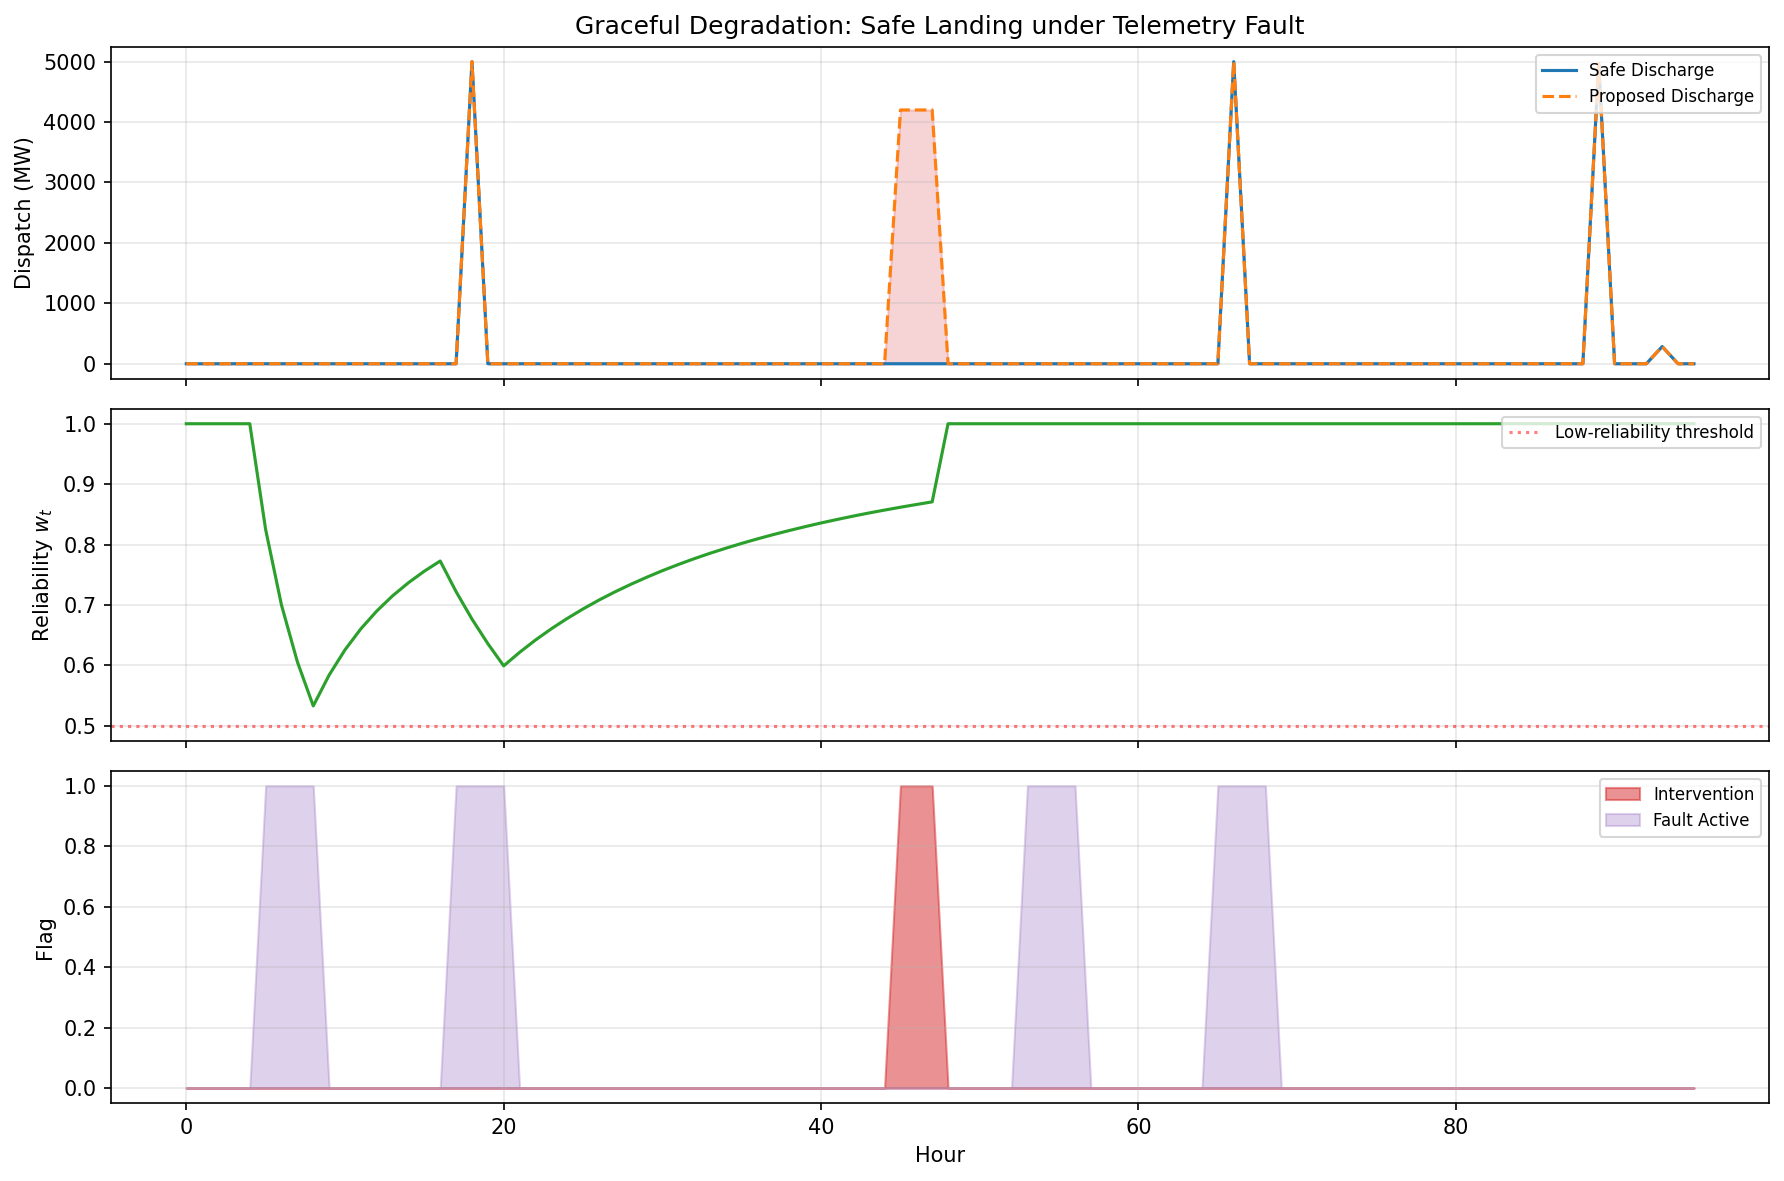
\includegraphics[width=0.85\textwidth]{reports/hil/fig_safe_landing_trace.png}
\caption{SOC trajectory during safe-landing activation (sudden blackout at $t=72$).
  The landing controller (blue) converges to the safe zone within 8~steps,
  while the unprotected controller (red dashed) drifts below SOC$_{\min}$.}
\label{fig:safe-landing-trace}
\end{figure}

\section{Formal Guarantee}

\begin{proposition}[Landing convergence]
\label{prop:landing-convergence}
Under the sub-Gaussian drift assumption and bounded power constraints,
the safe-landing protocol reaches $\mathcal{X}_{\text{safe}}$ in at most
\[
  T_L \;\le\; \left\lceil\,\frac{|x_t - x_{\text{mid}}|}
  {\eta_{\min} \cdot \Delta t}\,\right\rceil
\]
steps, where $\eta_{\min} = \min(P_{\max}^{\text{chg}},\, P_{\max}^{\text{dis}})$
and $x_{\text{mid}} = (\text{SOC}_{\min} + \text{SOC}_{\max})/2$.
\end{proposition}

\section{Summary}

The safe-landing protocol gives the battery stack an explicit degraded-mode
controller instead of relying only on implicit projection clipping.  The
current locked trace package supports the bounded claim that the battery can
enter a conservative landing behavior under severe observation loss; future
work can expand this into a broader family of runtime studies.
